\documentclass[../main.tex]{subfiles}

\begin{document}
    \subsection{Overview}
    Se desarrolla una aplicación móvil para iOS para la extracción de características que serán usadas en el entrenamiento de un modelo de Deep Learning.
    
    Está desarrollada en Swift 5 y será compatible con iPhone. El caso de uso de la aplicación será el siguiente:
    
    La aplicación realizará una llamada a un endpoint del API REST en un entorno local y obtendrá como respuesta un listado en formato JSON de las imágenes del dataset. El listado consiste en un diccionario en el cual por cada letra que se va a interpretar tendrá un listado de imágenes que representan esa letra.
    
    
    Por cada url obtenida, se descarga la imagen y se utilizará Vision Framework para obtener una predicción que consiste en detectar si existe una mano en la imagen, en caso de que exista, obtendremos como resultado las coordenadas de varias posiciones de la mano. Estas coordenadas incluyen la posición de la muñeca, y 4 posiciones de cada uno de los dedos, desde la punta del dedo hasta la parte inferior.
    
    Para cada conjunto de coordenadas que representan las posiciones de los dedos, se realiza un proceso de normalización. Este proceso persigue dos objetivos:
    
    \begin{enumerate}
        \item Lo importante de la posición de la mano no es en qué punto de la imagen está localizada, no importa si está en la parte superior de la imagen o en la parte inferior, sino lo importante es la posición relativa entre los dedos. Por tanto, el objetivo es que la misma posición de los dedos, sin importar en qué posición de la imagen esté localizada, tenga las mismas coordenadas.
        \item Evitar que las coordenadas  sean números demasiado pequeños porque dificultará el entrenamiento de un modelo de Deep Learning. Vamos a normalizar las coordenadas de la mano entre los valores 0.0 y 1.0, Siempre tendremos un punto de la mano que representará el valor 0.0 y otro punto de la mano que representará el valor 1.0, para ambos ejes de coordenadas.

    \end{enumerate}
    
    Una vez procesadas todas las imágenes y obtenidas sus características, se procede a almacenarlas en disco en ficheros con formato csv. La organización de los ficheros se muestra en la figura \ref{figure5}:
    
    \begin{figure}[h]
    \centering 
    \includegraphics[width=0.6\textwidth]{images/trainingapp/estructura-training-results.PNG}
    \caption{Estructura de los resultados de la extracción de características.}
    \label{figure5}
    \end{figure}
    
    Por último, se muestra la opción de compartir los resultados obtenidos, se utiliza esta función para comprimir y descargar los resultados obtenidos. Se podrán descargar por email, Airdrop o cualquier otra aplicación compatible en iOS.
    
\subsection{Arquitectura}

La aplicación seguirá la arquitectura MVVM: Model-View-ViewModel. Constará de una única pantalla y la aplicación cuenta con los siguientes componentes:

\begin{enumerate}
    \item ExtractFeaturesPicturesVC, ExtractFeaturesPicturesView: Se encargará de la interfaz, se comunica únicamente con el ViewModel.
    \item ExtractFeaturesPicturesViewModel: Será el ViewModel de la aplicación. Se encarga de comunicarse con diferentes workers que realizarán el trabajo de procesamiento de las imágenes y ficheros, y comunicará los resultados a la vista.
    \item Hand, Finger: Son los modelos de la aplicación. Ambos realizarán el proceso de convertir los resultados obtenidos a través de Vision framework en las coordenadas normalizadas que van a ser usadas para el entrenamiento del modelo. 
    \item VisionProcessImage, ApiManager, FileWorker: se encargan de realizar el procesamiento y coordinación de las operaciones a realizar, desde comunicarse con el API REST hasta almacenar los resultados obtenidos. 
\end{enumerate}

\subsection{Interfaz}

La interfaz se puede encontrar en los siguientes estados:

\begin{enumerate}
    \item Primer lanzamiento de la aplicación. La única opción posible es empezar con la extracción de las características \ref{figure6}.
    \item Extracción de las características en proceso \ref{figure7}.
    \item Tras finalizar la extracción de características podemos descargar los resultados por diferentes medios \ref{figure8}.
    \item En un lanzamiento posterior, podemos empezar otro entrenamiento o descargar los resultados de una ejecución anterior \ref{figure9}.
\end{enumerate}

\begin{figure}[h]
    \centering 
    \includegraphics[width=0.6\textwidth]{images/trainingapp/trainingapp1.PNG}
    \caption{Primer lanzamiento de la aplicación.}
    \label{figure6}
    \end{figure}
    
    \begin{figure}[h]
    \centering 
    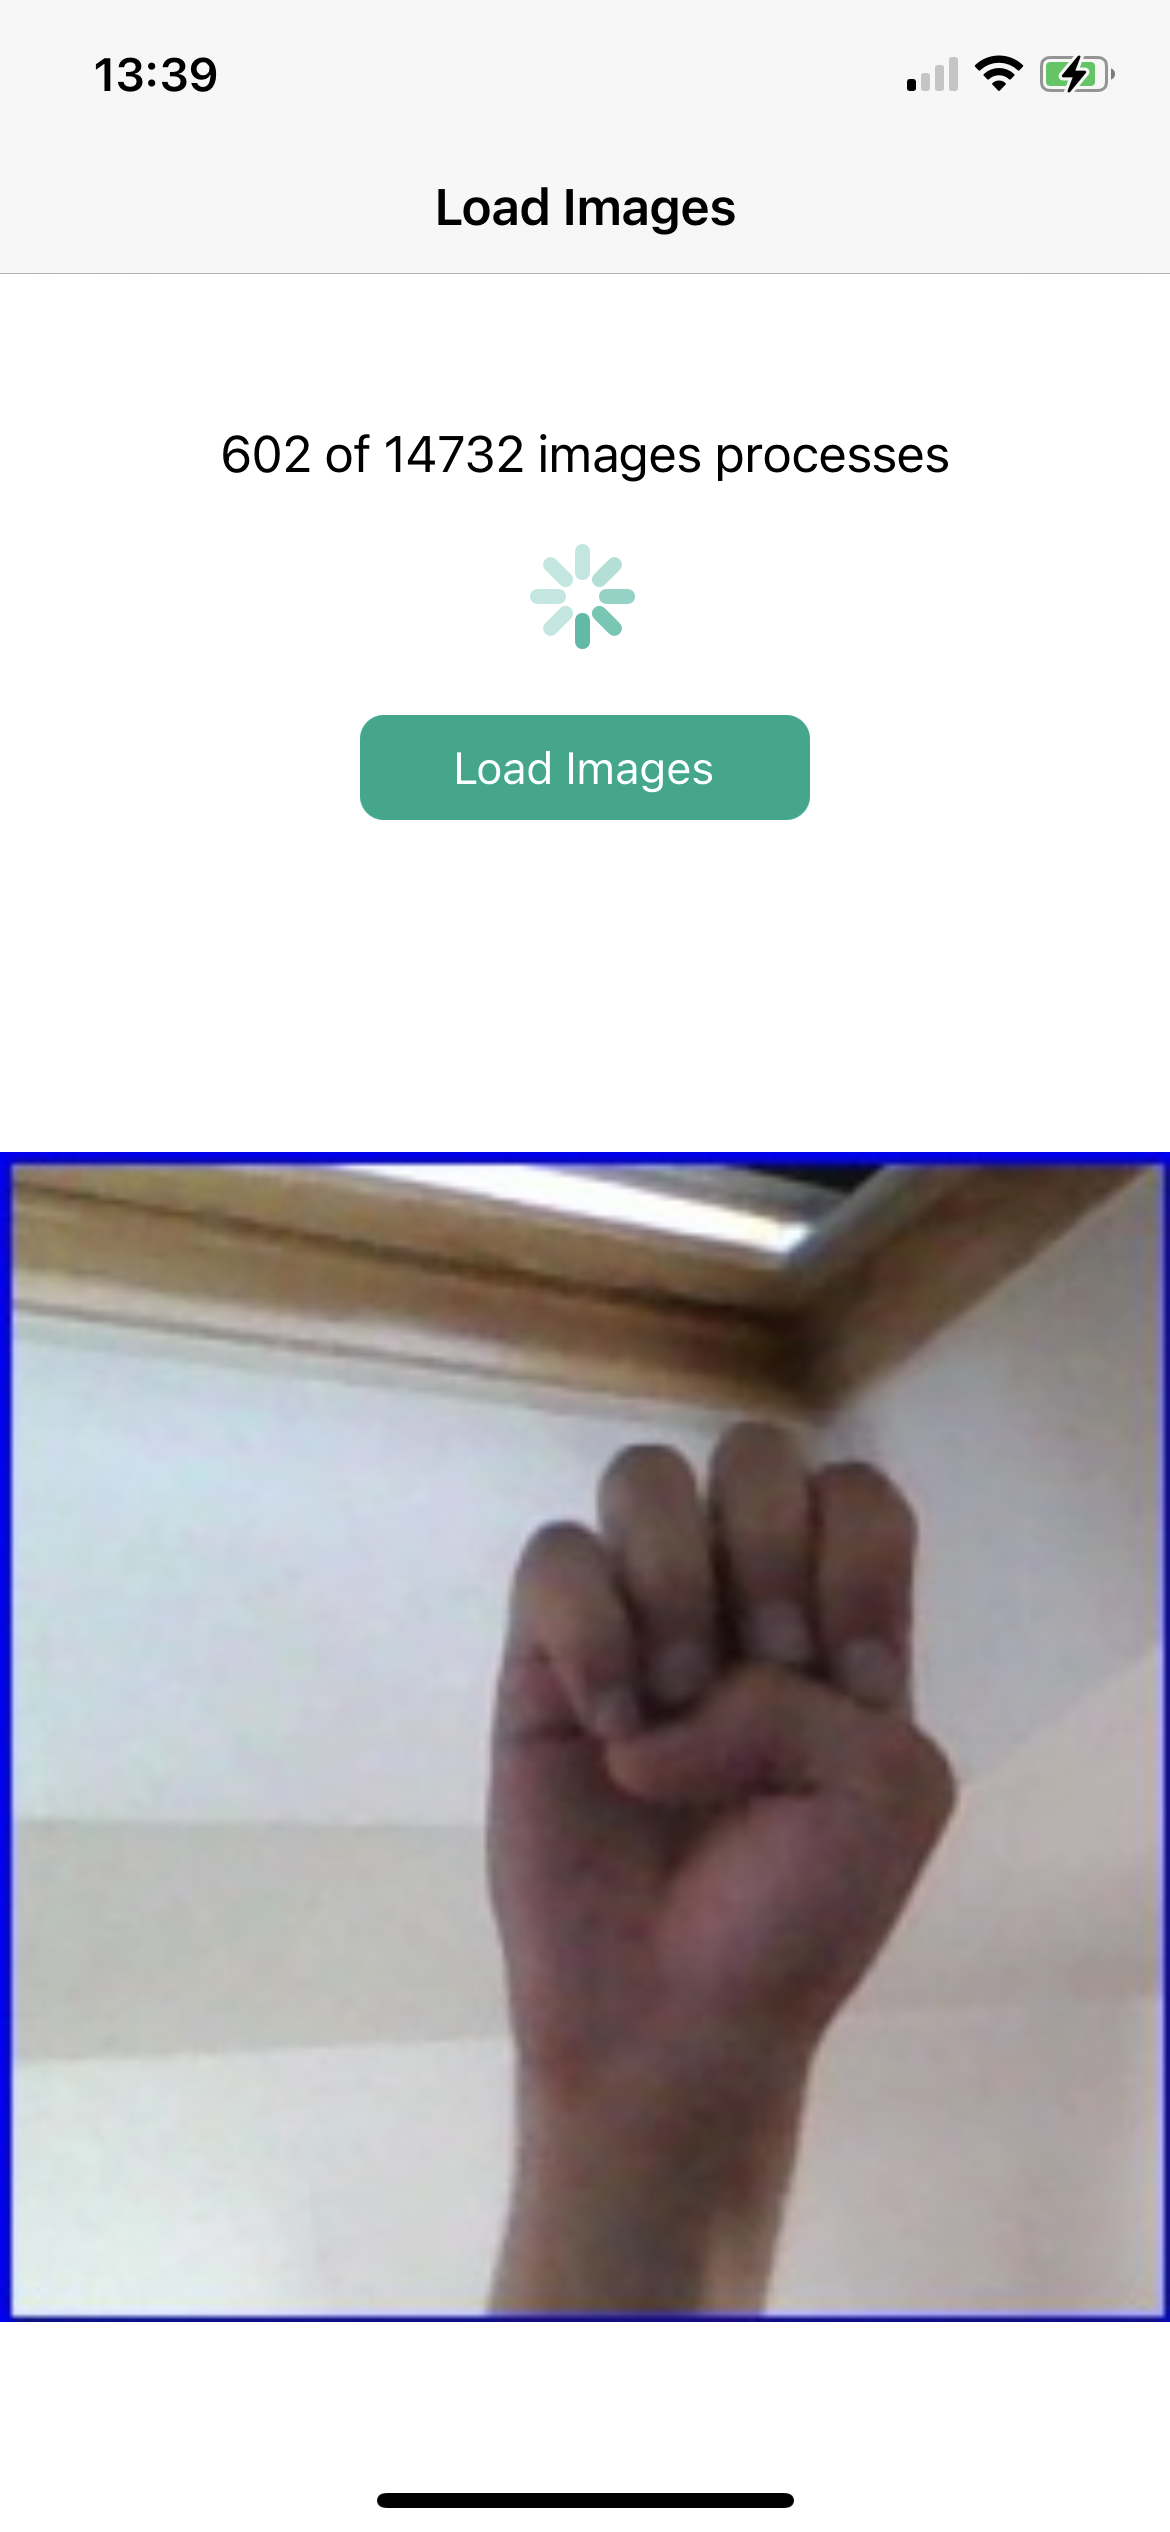
\includegraphics[width=0.6\textwidth]{images/trainingapp/trainingapp2.PNG}
    \caption{Entrenamiento en proceso.}
    \label{figure7}
    \end{figure}
    
    \begin{figure}[h]
    \centering 
    \includegraphics[width=0.6\textwidth]{images/trainingapp/trainingapp3.PNG}
    \caption{Descargar resultados.}
    \label{figure8}
    \end{figure}
    
    \begin{figure}[h]
    \centering 
    \includegraphics[width=0.6\textwidth]{images/trainingapp/trainingapp4.PNG}
    \caption{Pantalla inicial tras existir un entrenamiento previo.}
    \label{figure9}
    \end{figure}
    
\subsection{VNDetectHumanHandPoseRequest}

El código completo del proyecto es bastante amplio así que este documento se centra en las dos partes más importante que es la detección y normalización de coordenadas de los dedos de una mano. Para la detección de los dedos, se utiliza Vision Framework, y más específicamente, se utiliza VNDetectHumanHandPoseRequest \cite{handposerequest}.

VNDetectHumanHandPoseRequest detectará si existe una mano en una imagen, y en caso de que exista, se obtienen los siguientes resultados.

Como se puede ver en la figura \ref{figure10}, podemos obtener un total de 21 posiciones de la mano, 4 por cada uno de los dedos y una por la muñeca. Para cada posición, tendremos dos coordenadas representando cada eje, este nos deja con 42 coordenadas, que serán las características que usaremos para entrenar el modelo.

En las figuras \ref{figure11}, \ref{figure12}, \ref{figure13}, se muestra con más detalle las diferentes posiciones que se obtienen como resultado, las imágenes y más información relativa a VNDetectHumanHandPoseRequest puede encontrarse en la siguiente documentación \cite{wwdchandpose}.


\begin{figure}[h]
\centering 
\includegraphics[width=0.9\textwidth]{images/trainingapp/handpose/hanpose1.png}
\caption{Hand Landmarks.}
\label{figure10}
\end{figure}

\begin{figure}[h]
\centering 
\includegraphics[width=0.9\textwidth]{images/trainingapp/handpose/handpose2.png}
\caption{Index finger.}
\label{figure11}
\end{figure}

\begin{figure}[h]
\centering 
\includegraphics[width=0.9\textwidth]{images/trainingapp/handpose/handpose3.png}
\caption{Ring finger.}
\label{figure12}
\end{figure}

\begin{figure}[h]
\centering 
\includegraphics[width=0.9\textwidth]{images/trainingapp/handpose/handpose4.png}
\caption{Thumb finger.}
\label{figure13}
\end{figure}
    
Tras aplicar VNDetectHumanHandPoseRequest a una imagen, obtendremos una objeto de tipo VNHumanHandPoseObservation, del que extraemos las coordenadas para cada una de 21 posiciones de los dedos y muñeca. La siguiente función se encarga de convertir VNHumanHandPoseObservation en un objeto HandFingerPoints que se encarga de la normalización de coordenadas.

\begin{lstlisting}[style=swift]
func processObservations(_ observation: VNHumanHandPoseObservation) -> Hand? {
    guard observation.confidence >= minConfidenceObservation else {
        print("observation low confidence")
        return nil
    }
    
    do {
        let wrist = try observation.recognizedPoint(.wrist)
        let indexFingerPoints = try observation.recognizedPoints(.indexFinger)
        let ringFingerPoints = try observation.recognizedPoints(.ringFinger)
        let thumbFingerPoints = try observation.recognizedPoints(.thumb)
        let littleFingerPoints = try observation.recognizedPoints(.littleFinger)
        let middleFingerPoints = try observation.recognizedPoints(.middleFinger)
        
        let hand = HandFingerPoints(indexFingerPoints: indexFingerPoints,
                                    ringFingerPoints: ringFingerPoints,
                                    littleFingerPoints: littleFingerPoints,
                                    middleFingerPoints: middleFingerPoints,
                                    thumbFingerPoints: thumbFingerPoints,
                                    wristPoint: wrist)
        hand.normalizeHand()
        numberOfProcess += 1
        return hand
    } catch {
        print(error)
        return nil
    }
}
\end{lstlisting}

\subsection{HandFingerPoints}

Es el modelo que representa una mano. Se inicializa con las coordenadas de 21 posiciones de la mano, y se encarga de normalizar estas coordenadas y devolver los datos que serán almacenados como una interpretación de una letra formada por 42 números entre 0.0 y 1.0.

Cada posición está representada por una coordenada X y una coordenada Y. El proceso de normalización de coordenadas cuenta con dos fases para cada una de las coordenadas:

\begin{itemize}
    \item Transformar a coordenadas relativas: En el caso de la coordenada X, detectamos cual es el mínimo de todas las coordenadas X de la mano, este punto será el punto 0.0, y al resto de las coordenadas le restamos la diferencia entre el punto 0.0 original de la imagen y el que se ha establecido. De esta forma, no importa donde esté situada la mano en la imagen, lo que importa es cómo se relacionan las posiciones de los dedos entre sí. Se aplica para las coordenadas X e Y detectando cada una su mínimo en su eje. Esta será la función encargada de ello para cada dedo (4 puntos por cada dedo):
    
\begin{lstlisting}[style=swift]
func translatesToRelative(minX: Double, minY: Double) {
    if let point = tip {
        let x = point.x - minX
        let y = point.y - minY
        self.tip = VNPoint(x: x, y: y)
    }
    
    if let point = dip {
        let x = point.x - minX
        let y = point.y - minY
        self.dip = VNPoint(x: x, y: y)
    }
    
    if let point = pip {
        let x = point.x - minX
        let y = point.y - minY
        self.pip = VNPoint(x: x, y: y)
    }
    
    if let point = mcp {
        let x = point.x - minX
        let y = point.y - minY
        self.mcp = VNPoint(x: x, y: y)
    }
}
\end{lstlisting}
    \item Normalizar entre 0.0 y 1.0: En el caso de la coordenada X, la menor posición de todos los puntos siempre tendrá el valor 0.0, y la mayor posición el valor 1.0. Esto incrementa las diferencias entre los dedos de forma que puedan ser más visibles para el modelo de Deep Learning. Para ello, se detectan los mínimos y los máximos de cada eje, se calculan las diferencias entre ellos, y a cada punto se le resta el mínimo de sus eje y se divide por la diferencia entre el máximo y el mínimo. Se puede ver con más detalle en la siguiente función, que se encarga de normalizar las coordenadas de un dedo:

\begin{lstlisting}[style=swift]
func normalizeFinger(minX: Double, minY: Double, maxX: Double, maxY: Double) {
    let divideX = maxX - minX
    let divideY = maxY - minY
    
    if let point = tip {
        let x = (point.x - minX) / divideX
        let y = (point.y - minY) / divideY
        self.tip = VNPoint(x: x, y: y)
    }
    
    if let point = dip {
        let x = (point.x - minX) / divideX
        let y = (point.y - minY) / divideY
        self.dip = VNPoint(x: x, y: y)
    }
    
    if let point = pip {
        let x = (point.x - minX) / divideX
        let y = (point.y - minY) / divideY
        self.pip = VNPoint(x: x, y: y)
    }
    
    if let point = mcp {
        let x = (point.x - minX) / divideX
        let y = (point.y - minY) / divideY
        self.mcp = VNPoint(x: x, y: y)
    }
}
\end{lstlisting}
\end{itemize}

Tras este proceso de normalización de coordenadas, la última función de este modelo es devolver un vector de tipo Double que esté formado por 42 valores entre 0.0 y 1.0 que representan una letra. Este vector será almacenado en un fichero, en el que cada línea del fichero contiene una lista de 42 valores que representan una letra. Por cada letra, tendremos un fichero en formato csv en el que cada línea está formada por 42 valores que representan la misma letra tomada de una imagen diferente. Estos serán los datos que utilizaremos para entrenar un modelo de Deep Learning.

Se muestra una parte del código en la siguiente función, en el que se extraen las coordenadas normalizadas de cada uno de los dedos así como de la muñeca, y en el caso de que todos los valores serán correctos, se forma un vector con todos ellos:


\begin{lstlisting}[style=swift]
/// extract the location of all position in the hand if there is not null data
/// - Returns: 42 values array with the relatives coordinates of each position of the hand
func extractIfValidFeatures() -> [Double]? {
    guard let featuresIndex = indexInfo.extractIfValidFeatures(),
          let featuresRing = ringInfo.extractIfValidFeatures(),
          let featuresLittle = littleInfo.extractIfValidFeatures(),
          let middleInfo = middleInfo.extractIfValidFeatures(),
          let thumbInfo = thumbInfo.extractIfValidFeatures(),
          let wristInfo = wrist.extractIfValidFeatures() else {
        print("No valid hand")
        return nil
    }
    
    var result = [Double]()
    result.append(contentsOf: featuresIndex)
    result.append(contentsOf: featuresRing)
    result.append(contentsOf: featuresLittle)
    result.append(contentsOf: middleInfo)
    result.append(contentsOf: thumbInfo)
    result.append(contentsOf: wristInfo)
    return result
}
\end{lstlisting}

Parte de este código será también usado en la aplicación para interpretar ASL, en la aplicación de entrenamiento se utiliza este modelo para obtener las características que serán usadas para entrenar un modelo de Deep Learning. En la aplicación para interpretar ASL, estos datos serán la entrada  del modelo de Deep learning, el cual nos devolverá una predicción sobre los datos de entrada.

\end{document}


